\documentclass{article}
\usepackage[margin=1in]{geometry}
\usepackage{float}
\usepackage{listings}
\usepackage{xcolor}
\usepackage{graphicx}
\usepackage{amsmath} 
\usepackage{amssymb}

\definecolor{codegreen}{rgb}{0,0.6,0}
\definecolor{codegray}{rgb}{0.5,0.5,0.5}
\definecolor{codepurple}{rgb}{0.58,0,0.82}
\definecolor{backcolour}{rgb}{0.95,0.95,0.92}

\lstdefinestyle{mystyle}{
    backgroundcolor=\color{backcolour},   
    commentstyle=\color{codegreen},
    keywordstyle=\color{magenta},
    numberstyle=\tiny\color{codegray},
    stringstyle=\color{codepurple},
    basicstyle=\ttfamily\footnotesize,
    breakatwhitespace=false,         
    breaklines=true,                 
    captionpos=b,                    
    keepspaces=true,                 
    numbers=left,                    
    numbersep=5pt,                  
    showspaces=false,                
    showstringspaces=false,
    showtabs=false,                  
    tabsize=2
}
\lstset{style=mystyle}

\title{
    \vspace{-2cm}
    \Large Data Engineering 424 \\
    \Large Practical Assignment: Learning with Latent Random Variables\\
}
\author{
    Jacob Johannes Mostert \\ 
    27038122
}

\begin{document}
\maketitle

\section{Introduction}
In the prac we look at the Expectation-Maximisation (EM) algorithm for parameter estimation when latent variables are present. We focus on a regression problem where data points are generated by multiple lines, but the association between each point and its source line is unknown. We derive the updates for the algorithm, implement it in Python, and conduct experiments to see how initialisation, noise, data volume, and geometric arrangement affect the model's performance.

\section{Question 1: EM for a Regression Example with Multiple Lines}

In this section, we apply the Expectation-Maximisation (EM) algorithm to estimate the parameters of multiple lines when the association between data points and lines is unknown. Since the association variables are latent, we must iteratively alternate between estimating the responsibilities (E-step) and updating the line parameters (M-step) until the system converges.

\subsection{Outline of the Derivation for Question 1(a)}

The goal of the M-step is to find the updated parameters $\Theta^{new}$ that maximize the auxiliary function $\mathcal{Q}(\Theta)$. Because each term in $\mathcal{Q}(\Theta)$ only depends on the parameters of a single line, we can optimize the parameters for each line $l$ independently.

The relevant portion of the auxiliary function for a single line $l$ is given by:

$$
\mathcal{Q}_l = \sum_{m=1}^{M} \gamma_l^{[m]} \left( -\frac{1}{2\sigma_v^2} \left[ \hat{y}^{[m]} - (1-\alpha^{[m]})y_I^l - \alpha^{[m]}y_F^l \right]^2 \right)
$$

To find the maximum, we must take the partial derivatives of $\mathcal{Q}_l$ with respect to the two unknown parameters, $y_I^l$ and $y_F^l$, and set them to zero. 

First, we take the partial derivative with respect to $y_I^l$:

$$
\frac{\partial \mathcal{Q}_l}{\partial y_I^l} = \sum_{m=1}^{M} \gamma_l^{[m]} \left( -\frac{1}{2\sigma_v^2} \right) 2 \left[ \hat{y}^{[m]} - (1-\alpha^{[m]})y_I^l - \alpha^{[m]}y_F^l \right] (-(1-\alpha^{[m]})) = 0
$$

We can eliminate the constant multipliers and expand the equation to separate the known variables from the unknown parameters:

$$
y_I^l \sum_{m=1}^{M} \gamma_l^{[m]} (1-\alpha^{[m]})^2 + y_F^l \sum_{m=1}^{M} \gamma_l^{[m]} (1-\alpha^{[m]})\alpha^{[m]} = \sum_{m=1}^{M} \gamma_l^{[m]} (1-\alpha^{[m]})\hat{y}^{[m]}
$$

Next, we take the partial derivative with respect to $y_F^l$:

$$
\frac{\partial \mathcal{Q}_l}{\partial y_F^l} = \sum_{m=1}^{M} \gamma_l^{[m]} \left( -\frac{1}{2\sigma_v^2} \right) 2 \left[ \hat{y}^{[m]} - (1-\alpha^{[m]})y_I^l - \alpha^{[m]}y_F^l \right] (-\alpha^{[m]}) = 0
$$

By setting this to zero and rearranging in the same manner, we get:

$$
y_I^l \sum_{m=1}^{M} \gamma_l^{[m]} \alpha^{[m]} (1-\alpha^{[m]}) + y_F^l \sum_{m=1}^{M} \gamma_l^{[m]} (\alpha^{[m]})^2 = \sum_{m=1}^{M} \gamma_l^{[m]} \alpha^{[m]}\hat{y}^{[m]}
$$

We now have a system of two linear equations with two unknowns. This can be expressed in the standard matrix form $A\theta = b$:

$$
\begin{bmatrix} 
\sum_{m=1}^{M} \gamma_l^{[m]} (1-\alpha^{[m]})^2 & \sum_{m=1}^{M} \gamma_l^{[m]} (1-\alpha^{[m]})\alpha^{[m]} \\ 
\sum_{m=1}^{M} \gamma_l^{[m]} \alpha^{[m]} (1-\alpha^{[m]}) & \sum_{m=1}^{M} \gamma_l^{[m]} (\alpha^{[m]})^2 
\end{bmatrix} 
\begin{bmatrix} y_I^l \\ y_F^l \end{bmatrix} = 
\begin{bmatrix} 
\sum_{m=1}^{M} \gamma_l^{[m]} (1-\alpha^{[m]})\hat{y}^{[m]} \\ 
\sum_{m=1}^{M} \gamma_l^{[m]} \alpha^{[m]}\hat{y}^{[m]} 
\end{bmatrix}
$$

By solving this matrix equation for each line $l$, we obtain the new parameters $\Theta^{new}$ that maximize the auxiliary function for the current iteration.

\subsection{Overview of Implementation for Question 1(c)}

The EM algorithm was implemented in Python using the NumPy library to handle the matrix operations efficiently. The algorithm is broken down into two main functions: the E-step and the M-step.

\subsubsection*{The E-Step}
In the E-step, we calculate the responsibilities ($\gamma_l^{[m]}$), which represent the probability that a specific data point belongs to a specific line. We also implemented the Gaussian probability density function in NumPy. For each line, we calculate the expected $y$-value at each $\alpha$ position and determine the likelihood of the actual measurement. Finally, we normalize these likelihoods across all lines so they sum to 1.

\begin{lstlisting}[language=Python]
def gaussian_pdf(x, mean, std):
    variance = std ** 2
    coefficient = 1.0 / np.sqrt(2 * np.pi * variance)
    exponent = np.exp(-((x - mean) ** 2) / (2 * variance))
    return coefficient * exponent

def e_step(alpha, y_hat, y_I_est, y_F_est, sigma_v):
    L = len(y_I_est)
    M = len(alpha)
    probs = np.zeros((L, M))
    
    for l in range(L):
        mu_l = (1 - alpha) * y_I_est[l] + alpha * y_F_est[l]
        probs[l, :] = gaussian_pdf(y_hat, mu_l, sigma_v)
        
    # Normalize across lines (axis=0) to get responsibilities
    gamma = probs / np.sum(probs, axis=0)
    return gamma
\end{lstlisting}

\subsubsection*{The M-Step}
In the M-step, we update the coordinates for the start ($y_I$) and end ($y_F$) of each line. We achieve this by translating the system of linear equations derived in Question 1(a) directly into code. For each line, we construct the $2 \times 2$ matrix $A$ and the vector $b$ using the responsibilities calculated in the E-step. We then solve for the new parameters using \texttt{np.linalg.solve}.

\begin{lstlisting}[language=Python]
def m_step(alpha, y_hat, gamma):
    L = gamma.shape[0]
    y_I_new = np.zeros(L)
    y_F_new = np.zeros(L)
    
    for l in range(L):
        gamma_l = gamma[l, :]
        
        A11 = np.sum(gamma_l * (1 - alpha)**2)
        A12 = np.sum(gamma_l * (1 - alpha) * alpha)
        A22 = np.sum(gamma_l * alpha**2)
        A = np.array([[A11, A12], [A12, A22]])
        
        b1 = np.sum(gamma_l * (1 - alpha) * y_hat)
        b2 = np.sum(gamma_l * alpha * y_hat)
        b = np.array([b1, b2])
        
        theta_new = np.linalg.solve(A, b)
        y_I_new[l], y_F_new[l] = theta_new
        
    return y_I_new, y_F_new
\end{lstlisting}

\subsubsection*{Execution and Convergence}
The execution loop continuously alternates between these two steps. To determine when the algorithm has finished learning, we calculate the absolute difference between the old parameters and the newly calculated parameters. We sum the maximum shift on the left side and the maximum shift on the right side. If this total shift drops below a tiny tolerance threshold ($1 \times 10^{-4}$), we consider the algorithm converged and terminate the loop.

\begin{lstlisting}[language=Python]
for i in range(max_iters):
    gamma = e_step(alpha, y_hat, y_I_est, y_F_est, sigma_v)
    y_I_new, y_F_new = m_step(alpha, y_hat, gamma)
    
    # Check Convergence
    diff = np.max(np.abs(y_I_new - y_I_est)) + np.max(np.abs(y_F_new - y_F_est))
    
    if diff < tolerance:
        print(f"=== CONVERGED at iteration {i+1} ===")
        break
        
    y_I_est, y_F_est = y_I_new, y_F_new
\end{lstlisting}

\subsection{Question 1(d): Experimental Investigation of Algorithm Performance}
To understand the robustness and the limitations of the EM algorithm, we did several experiments by adjusting key parameters: initialization strategy, measurement noise ($\sigma_v$), number of observations ($M$), number of lines ($L$), and geometric arrangement. 

\subsubsection{Experiment 1: The Effect of Parameter Initialisation}
Because the EM algorithm is an iterative optimisation process, it tends to find local maxima. We tested this by simulating a crossing "X" dataset ($L=2$) with true coordinates ($y_I \in \{2.0, 7.0\}$, $y_F \in \{8.0, 3.0\}$) and testing two different initialisation strategies.

\begin{table}[H]
\centering
\begin{tabular}{|l|c|c|c|c|c|c|}
\hline
\textbf{Init Strategy} & \textbf{Line} & \textbf{Init $y_I$} & \textbf{Init $y_F$} & \textbf{Final $y_I$} & \textbf{Final $y_F$} & \textbf{Iterations} \\ \hline
Random Guesses & 1 & 3.9963 & 6.8560 & 1.7951 & 8.1392 & 7 \\ 
(\texttt{np.random}) & 2 & 8.6057 & 5.7893 & 7.0274 & 3.0994 & \\ \hline
Informed Guesses & 1 & 1.0000 & 9.0000 & 1.9462 & 7.9998 & 6 \\ 
(\texttt{np.linspace}) & 2 & 9.0000 & 1.0000 & 6.8871 & 3.2248 & \\ \hline
\end{tabular}
\caption{Results of random vs. informed parameter initialisation.}
\label{tab:init}
\end{table}

The algorithm converges quicker and more accurately when the initial parameters are reasonably chosen. The random initialisation led to a slower convergence and a final estimation that was less accurate (Appendix, Figure \ref{fig:random_init}). When an informed initialisation was used, the algorithm found the true crossing shape perfectly (Appendix, Figure \ref{fig:chosen_init}).

\subsubsection{Experiment 2: The Effect of Noise ($\sigma_v$)}
We held the number of measurements constant ($M=200$) and used true coordinates ($y_I \in \{2.0, 7.0\}$, $y_F \in \{8.0, 3.0\}$). We varied the noise standard deviation to observe how uncertainty impacts the E-step responsibilities.

\begin{table}[H]
\centering
\begin{tabular}{|l|c|c|c|c|}
\hline
\textbf{Noise Level ($\sigma_v$)} & \textbf{Line} & \textbf{Final $y_I$} & \textbf{Final $y_F$} & \textbf{Iterations} \\ \hline
Low Noise ($\sigma_v = 0.1$) & 1 & 1.9992 & 7.9992 & 3 \\ 
 & 2 & 6.9839 & 3.0445 & \\ \hline
High Noise ($\sigma_v = 2.0$) & 1 & 1.9860 & 7.8766 & 19 \\ 
 & 2 & 6.5942 & 4.1371 & \\ \hline
\end{tabular}
\caption{Algorithm convergence across varying levels of measurement noise.}
\label{tab:noise}
\end{table}

With low noise ($\sigma_v = 0.1$), the data points cluster tightly around their true lines. Thus, the likelihood calculations in the E-step return near-absolute certainties, allowing the M-step to update parameters perfectly in just 3 iterations (Appendix, Figure \ref{fig:low_noise}). With high noise ($\sigma_v = 2.0$), the points overlap significantly. The algorithm is forced to take small, uncertain steps, leading to 19 iterations and a final estimation that noticeably deviates from the true lines (Appendix, Figure \ref{fig:high_noise}).

\subsubsection{Experiment 3: The Effect of the Number of Measurements ($M$)}
To see if more data can combat noise, we locked the noise at $\sigma_v = 0.5$, kept true coordinates ($y_I \in \{2.0, 7.0\}$, $y_F \in \{8.0, 3.0\}$), and varied the number of observations $M$.

\begin{table}[H]
\centering
\begin{tabular}{|l|c|c|c|c|}
\hline
\textbf{Number of Points ($M$)} & \textbf{Line} & \textbf{Final $y_I$} & \textbf{Final $y_F$} & \textbf{Iterations} \\ \hline
Low Data ($M = 20$) & 1 & 1.5099 & 8.1507 & 5 \\ 
 & 2 & 7.0826 & 2.7816 & \\ \hline
Medium Data ($M = 200$) & 1 & 1.9462 & 7.9998 & 6 \\ 
 & 2 & 6.8871 & 3.2248 & \\ \hline
High Data ($M = 1000$) & 1 & 2.0071 & 7.9752 & 5 \\ 
 & 2 & 7.0553 & 3.0243 & \\ \hline
\end{tabular}
\caption{The effect of data volume on the stability of parameter estimation.}
\label{tab:measurements}
\end{table}

When $M=20$, random noisy outliers hold more weight. The algorithm overfits, leading to skewed final parameters (Appendix, Figure \ref{fig:m20}). Medium data ($M=200$) establishes a reasonable baseline (Appendix, Figure \ref{fig:m200}). However, as we scale up to $M=1000$, the great number of points penalises the impact of individual noisy outliers, guiding the M-step to a highly precise parameter estimation (Appendix, Figure \ref{fig:m1000}).

\subsubsection{Experiment 4: Number of Lines ($L$)}
We tested more complex environments. For $L=3$, true coordinates were ($y_I \in \{2.0, 4.5, 7.0\}$, $y_F \in \{8.0, 5.5, 3.0\}$). For $L=5$, true coordinates were ($y_I \in \{2.0, 3.25, 4.5, 5.75, 7.0\}$, $y_F \in \{8.0, 6.75, 5.5, 4.25, 3.0\}$).

\begin{table}[H]
\centering
\begin{tabular}{|l|c|c|}
\hline
\textbf{Configuration} & \textbf{Final Parameters ($y_I$, $y_F$)} & \textbf{Iterations} \\ \hline
$L = 3$ lines & Line 1: (2.1421, 7.9322) & 19 \\ 
($M=500$) & Line 2: (4.6071, 5.4691) & \\ 
 & Line 3: (6.9097, 3.1514) & \\ \hline
$L = 5$ lines & Line 1: (1.9617, 7.9480), Line 2: (3.3309, 6.8410) & 49 \\ 
($M=1000$) & Line 3: (4.6396, 5.3081), Line 4: (5.6483, 4.1042) & \\ 
 & Line 5: (7.1126, 3.0882) & \\ \hline
\end{tabular}
\caption{Convergence statistics for complex latent spaces.}
\label{tab:lines}
\end{table}

The algorithm successfully handled $L=3$ (Appendix, Figure \ref{fig:l3}) and $L=5$ (Appendix, Figure \ref{fig:l5}). As the number of lines increases, the algorithm requires more iterations to converge (49 iterations for $L=5$) because the E-step responsibilities are split between many similar candidates. To support higher $L$ values successfully, a proportionately higher $M$ value is necessary to provide enough data to separate the lines.

\subsubsection{Experiment 5: The Effect of Line Arrangement}
Finally, we tested how the physical arrangement of the true lines impacts the algorithm's ability to converge, specifically looking at a parallel arrangement with true coordinates ($y_I \in \{2.0, 5.0\}, y_F \in \{5.0, 8.0\}$).

\begin{table}[H]
\centering
\begin{tabular}{|l|c|c|c|c|c|c|}
\hline
\textbf{Init Strategy} & \textbf{Line} & \textbf{Init $y_I$} & \textbf{Init $y_F$} & \textbf{Final $y_I$} & \textbf{Final $y_F$} & \textbf{Iterations} \\ \hline
Parallel Init & 1 & 1.0000 & 1.0000 & 2.0127 & 5.0087 & 4 \\ 
 & 2 & 9.0000 & 9.0000 & 4.9032 & 8.2035 & \\ \hline
Crossing Init & 1 & 1.0000 & 9.0000 & 1.1810 & 9.1641 & 8 \\ 
 & 2 & 9.0000 & 1.0000 & 5.4680 & 4.2291 & \\ \hline
\end{tabular}
\caption{Algorithm performance on parallel true lines depending on initialisation topology.}
\label{tab:arrangement}
\end{table}

The geometry of the true data determines the complexity of the inference problem. When the true data was parallel, providing a parallel initialisation allowed the algorithm to converge almost immediately (Appendix, Figure \ref{fig:parallel_correct}). However, when we forced a crossing "X" initialisation onto the parallel data, the algorithm failed (Appendix, Figure \ref{fig:parallel_wrong}). The geometric mismatch caused the algorithm to find a local maximum. This shows a weakness of the EM algorithm: its success is greatly affected by providing a starting state that aligns with the true structure of the data.

\section{Conclusion}
The Expectation-Maximisation algorithm is an effective method for estimating parameters when latent variables are present. Our implementation successfully identified multiple hidden lines from noisy data. However, the experiments revealed clear limitations. The EM algorithm is highly sensitive to initialisation; a poor starting guess easily traps it in a local maximum. High measurement noise blurs data boundaries, while too few data points lead to overfitting. Providing a large volume of data helps smooth out noise. Finally, the algorithm relies heavily on distinct geometric separation and requires an initial guess that roughly matches the true shape of the data to guarantee successful convergence.

\newpage

\section{Question 2: Expectation-Maximization for Hamming (7,4) Code}
Please note that I did not extend the model to estimate the \textit{encoder error parameters} ($\theta_c$). Instead, I focused on the core EM algorithm for estimating the channel noise parameter $\theta_e$ assuming a perfect encoder. The Bayesian Network representation and the mathematical derivation of the EM updates are based on this.

\subsection{(a) Bayesian Network Representation}
The noisy communication channel can be modeled as a Bayesian Network, illustrating the conditional dependencies between the transmitted and received bits.

\begin{figure}[h!]
    \centering
    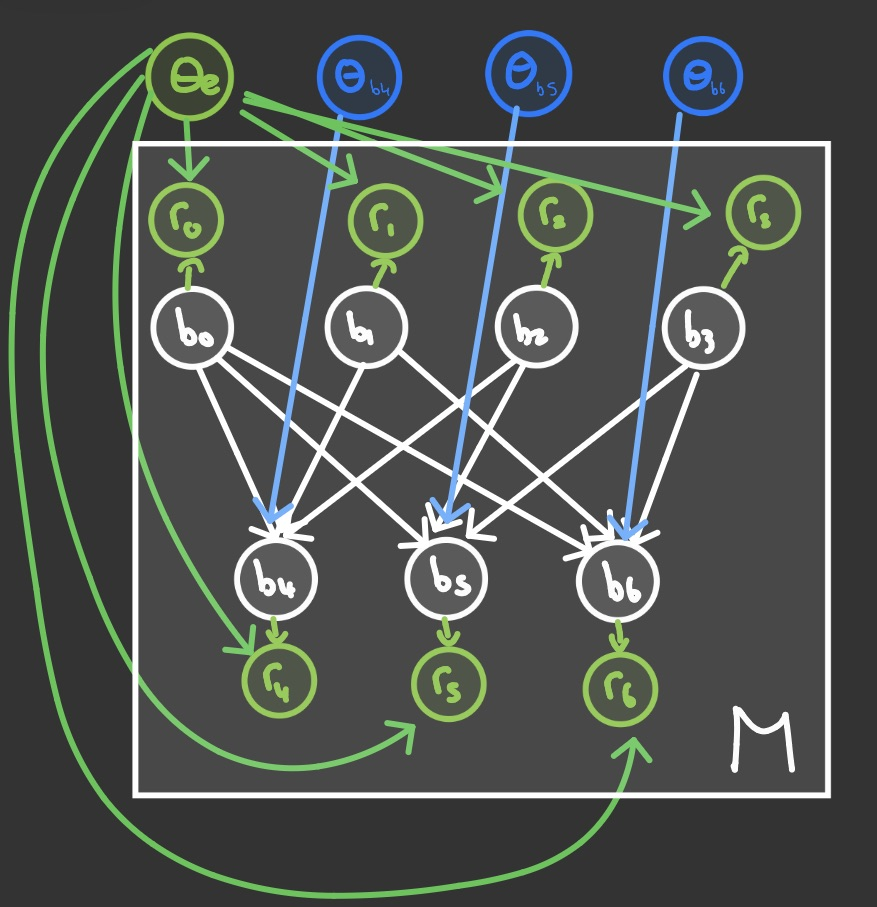
\includegraphics[width=0.6\textwidth]{images/BN.png}
    \caption{Bayesian Network for the Hamming (7,4) transmission (Blue shows encode error parameters which is not included in this model).}
    \label{fig:bn}
\end{figure}

As shown in Figure \ref{fig:bn}, the network consists of 14 total nodes per transmission block. The four original data bits ($b_0, b_1, b_2, b_3$) act as root nodes with independent priors. The three check bits ($b_4, b_5, b_6$) are completely determined by their respective data bit parents according to the even-parity rules. Finally, the seven received bits ($r_0, \dots, r_6$) are the only observed (green) variables, each depending solely on its corresponding transmitted bit, governed by the channel noise parameter $\theta_e$.

\subsection{(b) \& (c) Mathematical Derivation of the EM Algorithm}
The objective is to estimate the unknown channel error probability $\theta_e$ given only the noisy received bits. Because the transmitted bits ($\mathcal{H}$) are hidden, we utilize the Expectation-Maximization (EM) algorithm to maximize the incomplete-data log-likelihood.

The fundamental trick of the EM derivation relies on the factorization properties of the Bayesian Network. The joint probability of the entire network is the product of every node given its parents. When we construct the complete-data log-likelihood, the logarithm converts this massive product into a sum of independent local log-probabilities. 

In the E-step, we define the auxiliary function $\mathcal{Q}(\Theta)$ as the expected value of this log-likelihood with respect to the posterior distribution of the hidden variables, $q(\mathcal{H})$. Because the log-likelihood is a sum of local terms (each depending on only one transmitted bit), the expectation over the joint hidden state collapses into a sum over single-variable marginal probabilities. 

For the channel error parameter $\theta_e$, the relevant portion of the $\mathcal{Q}$ function simplifies to:
\begin{equation}
    \mathcal{Q}_{\theta_e}(\Theta) = \sum_{m=1}^{M} \sum_{i=0}^{6} \sum_{b_i^{[m]}} q\left(b_i^{[m]}\right) \log p\left(r_i^{[m]} \mid b_i^{[m]}; \theta_e\right)
\end{equation}

To simplify the maximization step, we can express this in terms of the expected number of correct bits ($\mathbb{E}[N_{correct}]$) and the expected number of errors ($\mathbb{E}[N_{error}]$) across the entire dataset:
\begin{equation}
    \mathcal{Q}_{\theta_e}(\Theta) = \mathbb{E}[N_{correct}] \log(1 - \theta_e) + \mathbb{E}[N_{error}] \log(\theta_e)
\end{equation}

In the M-step, we maximize this function by taking the partial derivative with respect to $\theta_e$ and setting it to zero:
\begin{equation}
    \frac{\partial \mathcal{Q}}{\partial \theta_e} = -\frac{\mathbb{E}[N_{correct}]}{1 - \theta_e} + \frac{\mathbb{E}[N_{error}]}{\theta_e} = 0
\end{equation}

Moving the negative term to the other side and cross-multiplying yields:
\begin{equation}
    \theta_e \cdot \mathbb{E}[N_{correct}] = (1 - \theta_e) \cdot \mathbb{E}[N_{error}]
\end{equation}

By expanding the right side and isolating $\theta_e$, we arrive at a highly intuitive update rule:
\begin{equation}
    \theta_e^{(new)} = \frac{\mathbb{E}[N_{error}]}{\mathbb{E}[N_{error}] + \mathbb{E}[N_{correct}]} = \frac{\mathbb{E}[N_{error}]}{7M}
\end{equation}
This proves that the new estimate for the channel noise is simply the expected number of bit errors divided by the total number of bits transmitted.

\subsection{(d) Implementation in C++ utilizing \texttt{emdw}}


\subsubsection*{The E-Step}
For a given iteration, the algorithm explicitly constructs the seven channel measurement factors utilizing the current estimate of $\theta_e$. The observed received bits for block $m$ are injected as evidence using \texttt{observeAndReduce}. These reduced factors are then absorbed into the base network to form the joint distribution, which is subsequently normalized. Finally, \texttt{marginalize} is called for each hidden bit $b_i$, and we extract the specific probability that $b_i = r_i$ (correct) and $b_i \neq r_i$ (error) using \texttt{potentialAt} to accumulate the expected counts.

\begin{lstlisting}[language=C++]
// Channel Factors (Using current est_theta_e)
double pc = 1.0 - est_theta_e;
double pe = est_theta_e;
rcptr<Factor> pR0_B0 = uniqptr<DT>(new DT({B0, R0}, {bDom, bDom}, defProb, {{{0,0}, pc}, {{0,1}, pe}, {{1,0}, pe}, {{1,1}, pc}}));
// ... (repeated for R1_B1 through R6_B6)

// Observe & Reduce
rcptr<Factor> red_pR0_B0 = pR0_B0->observeAndReduce({R0}, {T(D[m][0])});
// ... (repeated for R1 through R6)

// Joint Distribution
rcptr<Factor> jointRx = pB0->absorb(pB1)->absorb(pB2)->absorb(pB3)
                           ->absorb(pB4_B0B1B2)->absorb(pB5_B0B2B3)->absorb(pB6_B0B1B3)
                           ->absorb(red_pR0_B0)->absorb(red_pR1_B1)->absorb(red_pR2_B2)
                           ->absorb(red_pR3_B3)->absorb(red_pR4_B4)->absorb(red_pR5_B5)
                           ->absorb(red_pR6_B6)->normalize();

// Marginalize & Normalize (Example shown for B0)
rcptr<Factor> postB0 = jointRx->marginalize({B0})->normalize();

// Extract Probabilities
rcptr<DT> dtB0 = dynamic_pointer_cast<DT>(postB0);
E_N_correct += dtB0->potentialAt({B0}, {T(D[m][0])});
E_N_error += dtB0->potentialAt({B0}, {T(1 - D[m][0])});
\end{lstlisting}

\subsubsection*{The M-Step}
Once all $M$ blocks are processed, the accumulated expected errors are divided by the total of expected errors and correct bits to produce the updated $\theta_e$. This new parameter is fed into the next iteration until the absolute change drops below a tolerance of $1 \times 10^{-5}$.

\begin{lstlisting}[language=C++]
// M-STEP: Update parameters
est_theta_e = E_N_error / (E_N_error + E_N_correct);

cout << "Iteration " << iter + 1 << " - Estimated Theta_e: " << est_theta_e << endl;

if (abs(est_theta_e - old_theta_e) < tolerance) {
    cout << "=== CONVERGED at Iteration " << iter + 1 << " ===" << endl;
    break;
}
old_theta_e = est_theta_e;
\end{lstlisting}

\subsection{(e) Experimental Results and Initialization Variance}
The algorithm was tested by generating a dataset of $M=1000$  with a true channel noise of $\theta_e = 0.05$. 

When initialized with a reasonable guess (e.g., $\theta_e^{(init)} = 0.15$), the algorithm converged quickly.

To thoroughly evaluate the algorithm's robustness, we conducted two additional experiments varying the dataset size ($M$) and the initial parameter guess ($\theta_e^{(init)}$). The results are summarized in Table \ref{tab:q2_experiments}.

\begin{table}[H]
\centering
\begin{tabular}{|l|c|c|c|c|c|}
\hline
\textbf{Test Condition} & \textbf{Blocks ($M$)} & \textbf{Init $\theta_e$} & \textbf{True $\theta_e$} & \textbf{Final $\theta_e$} & \textbf{Iterations} \\ \hline
Baseline (Optimal) & 1000 & 0.15 & 0.05 & 0.0494 & 7 \\ \hline
Low Data Volume & 20 & 0.15 & 0.05 & 0.0314 & 6 \\ \hline
Inverted Initialization & 1000 & 0.60 & 0.05 & 0.9454 & 14 \\ \hline
\end{tabular}
\caption{The effect of dataset size and initialization on EM parameter estimation.}
\label{tab:q2_experiments}
\end{table}

\textbf{The Effect of Data Volume ($M = 20$):} 
When the dataset is reduced to just 20 blocks, the algorithm converges quickly but inaccurately (estimating $0.0314$ instead of $0.05$). This a variance issue. With only 140 total bits transmitted, the specific random noise generated for this small sample does not perfectly reflect the true 5\% error rate. The algorithm successfully finds the best explanation for the data it was given, but the data itself is too sparse to accurately represent the true channel distribution.

\textbf{The Effect of Initialization ($\theta_e^{(init)} = 0.6$):} 
The EM algorithm is very sensitive to local maxima. In our second experiment, we initialized the guess above the $0.5$ threshold. A channel error rate greater than $50\%$ implies that the channel is actively inverting the signal (flipping more bits than it leaves alone). Because the algorithm started with this assumption, it climbed the nearest gradient and converged to $0.9454$. The algorithm became "trapped" in a local maximum. This proves that for the Hamming (7,4) decoder to function, the initial guess must anchor the algorithm to the assumption that the majority of bits are transmitted correctly ($\theta_e < 0.5$).

\newpage
\appendix
\section{Appendix: Figures}

\begin{figure}[H]
\centering
\begin{minipage}{0.48\textwidth}
    \centering
    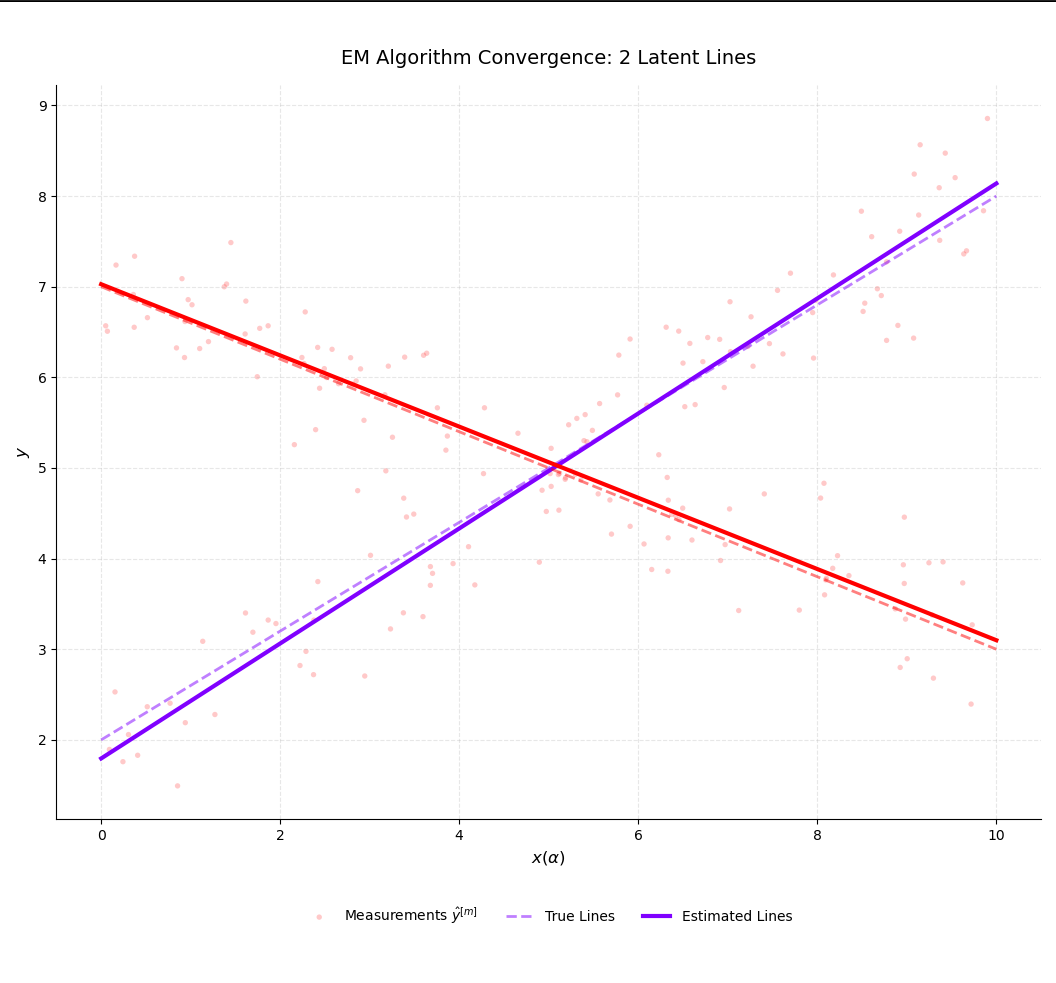
\includegraphics[width=\linewidth]{images/random.png}
    \caption{Random initialisation.}
    \label{fig:random_init}
\end{minipage}\hfill
\begin{minipage}{0.48\textwidth}
    \centering
    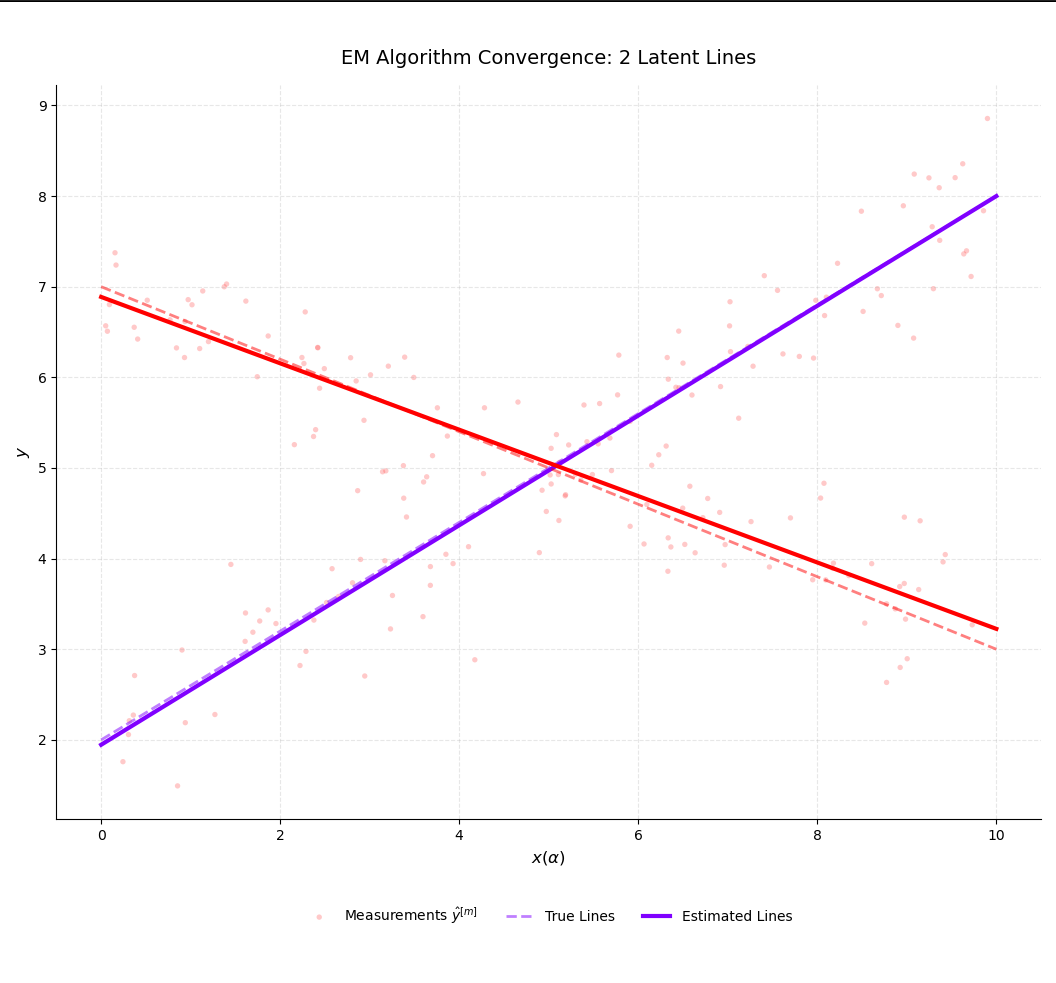
\includegraphics[width=\linewidth]{images/chosen.png}
    \caption{Informed initialisation.}
    \label{fig:chosen_init}
\end{minipage}
\end{figure}

\begin{figure}[H]
\centering
\begin{minipage}{0.48\textwidth}
    \centering
    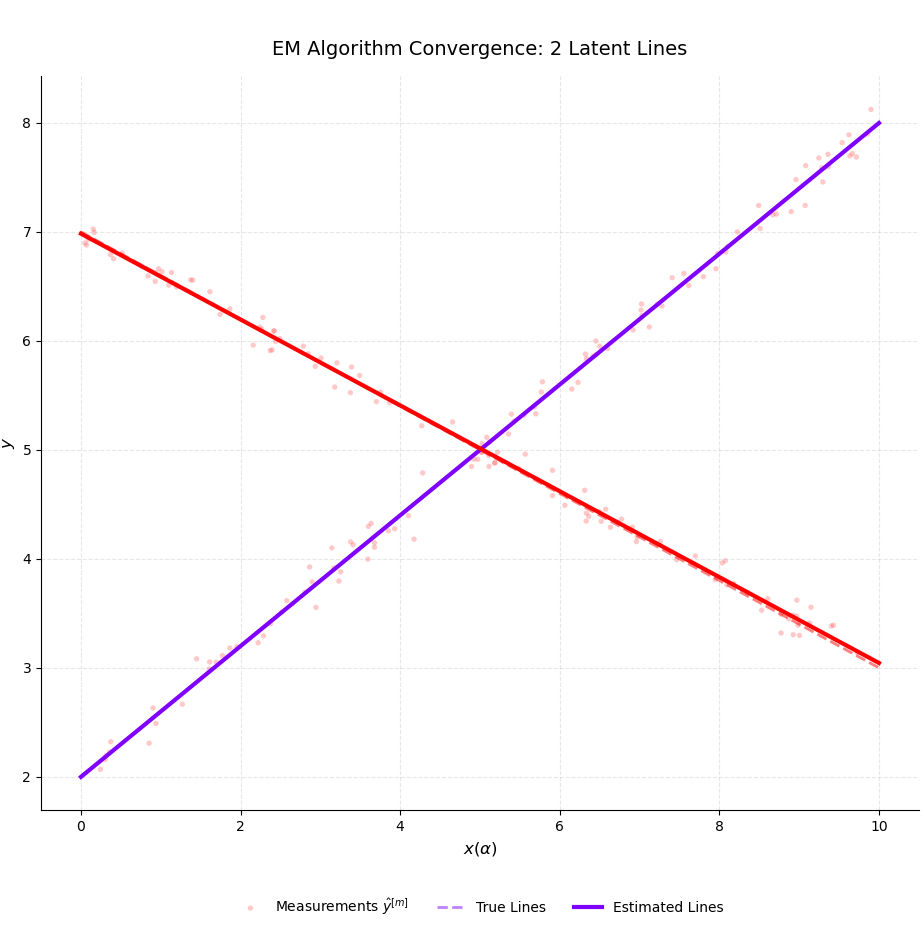
\includegraphics[width=\linewidth]{images/sigma1.png}
    \caption{Fast and highly accurate convergence with low noise ($\sigma_v = 0.1$).}
    \label{fig:low_noise}
\end{minipage}\hfill
\begin{minipage}{0.48\textwidth}
    \centering
    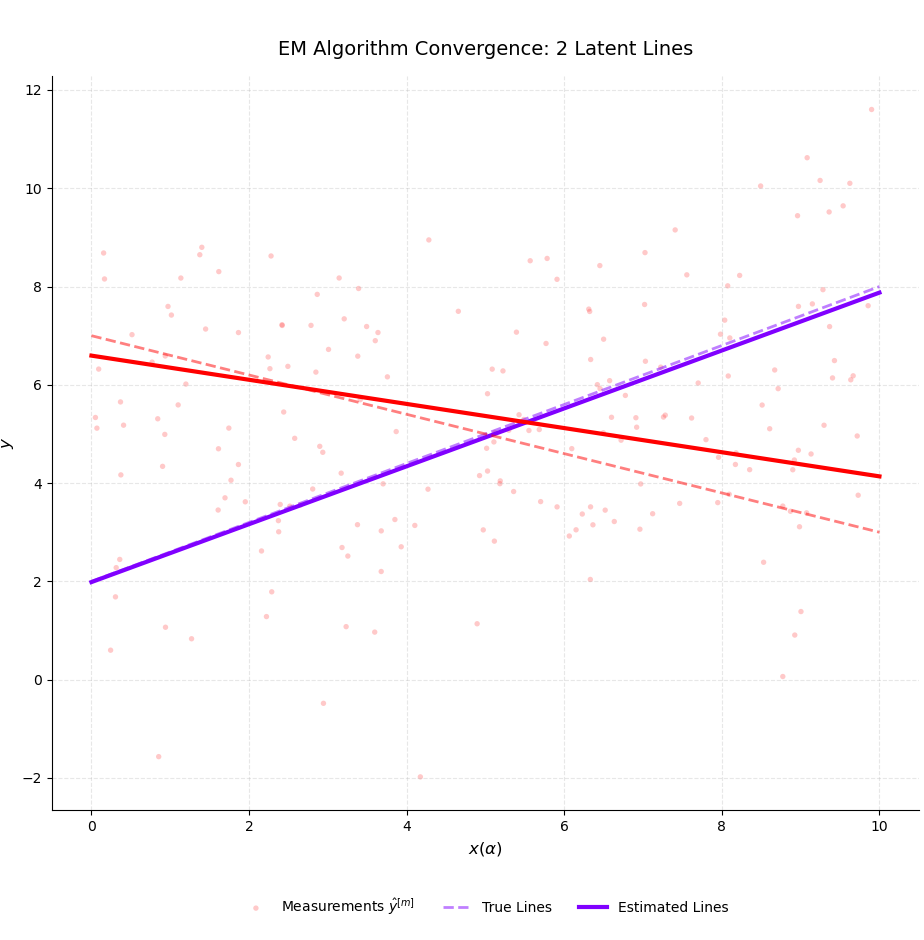
\includegraphics[width=\linewidth]{images/sigma2.png}
    \caption{Slower, less accurate convergence due to high noise ($\sigma_v = 2.0$).}
    \label{fig:high_noise}
\end{minipage}
\end{figure}

\begin{figure}[H]
\centering
\begin{minipage}{0.32\textwidth}
    \centering
    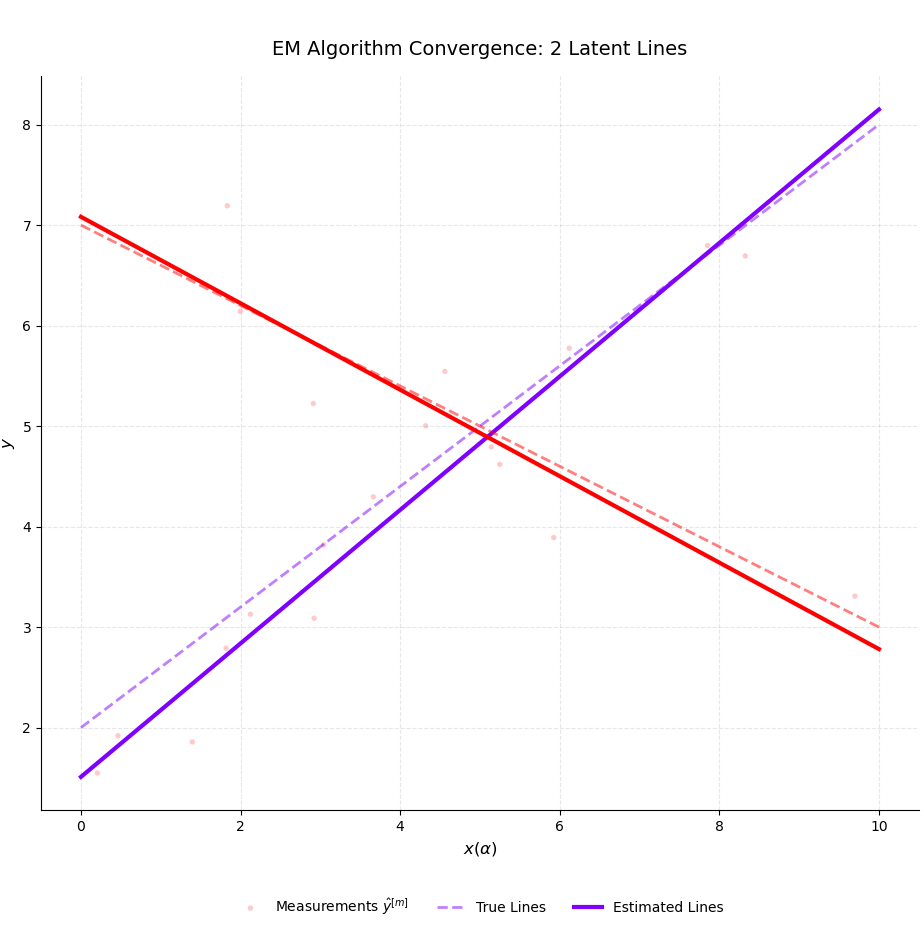
\includegraphics[width=\linewidth]{images/M1.png}
    \caption{$M=20$ (Overfitting)}
    \label{fig:m20}
\end{minipage}\hfill
\begin{minipage}{0.32\textwidth}
    \centering
    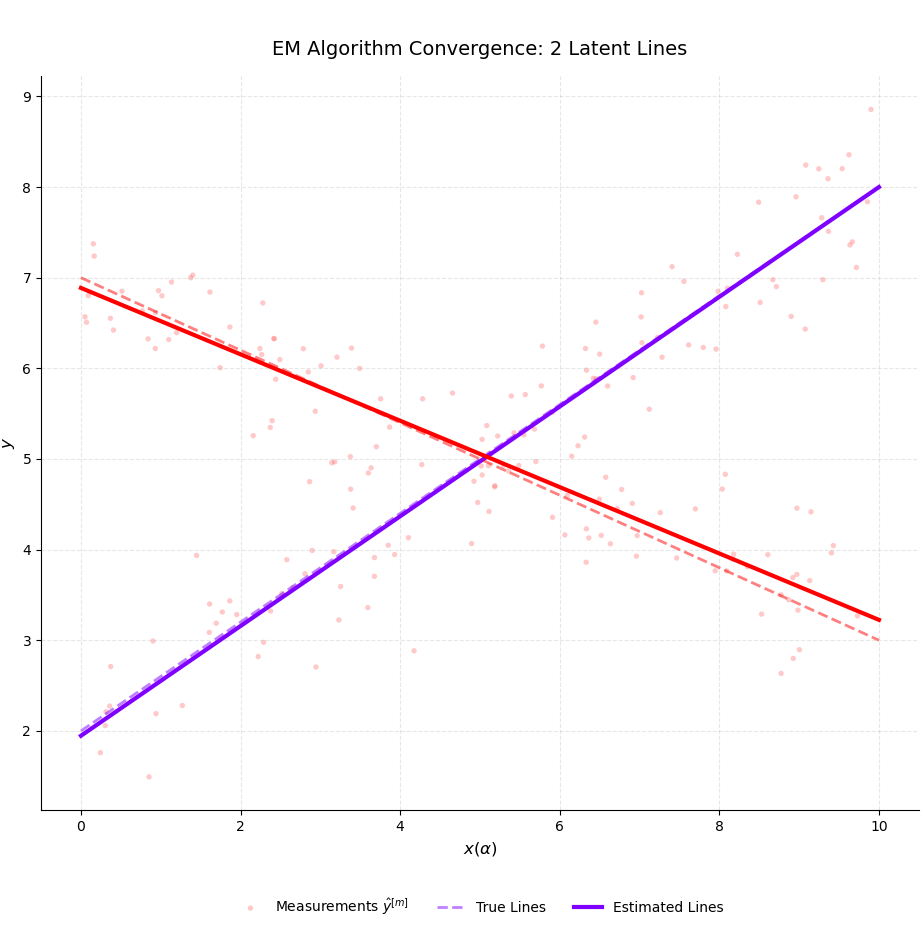
\includegraphics[width=\linewidth]{images/M2.png}
    \caption{$M=200$ (Baseline)}
    \label{fig:m200}
\end{minipage}\hfill
\begin{minipage}{0.32\textwidth}
    \centering
    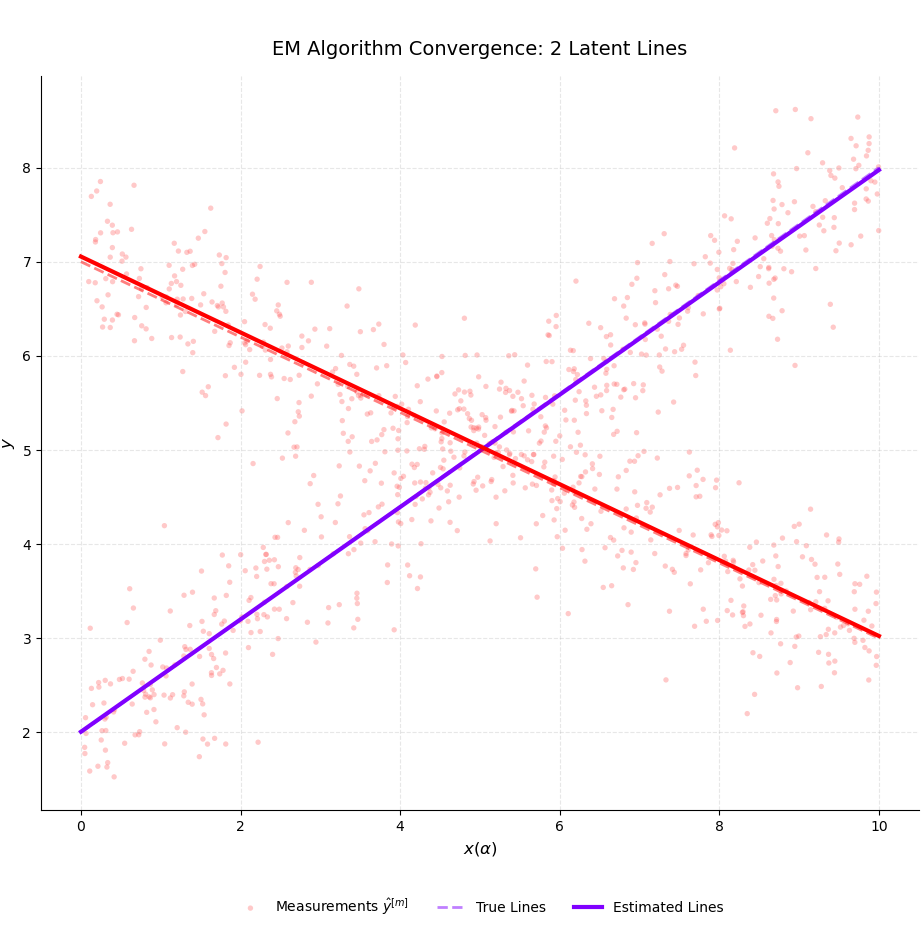
\includegraphics[width=\linewidth]{images/M3.png}
    \caption{$M=1000$ (Stable estimation)}
    \label{fig:m1000}
\end{minipage}
\end{figure}

\begin{figure}[H]
\centering
\begin{minipage}{0.48\textwidth}
    \centering
    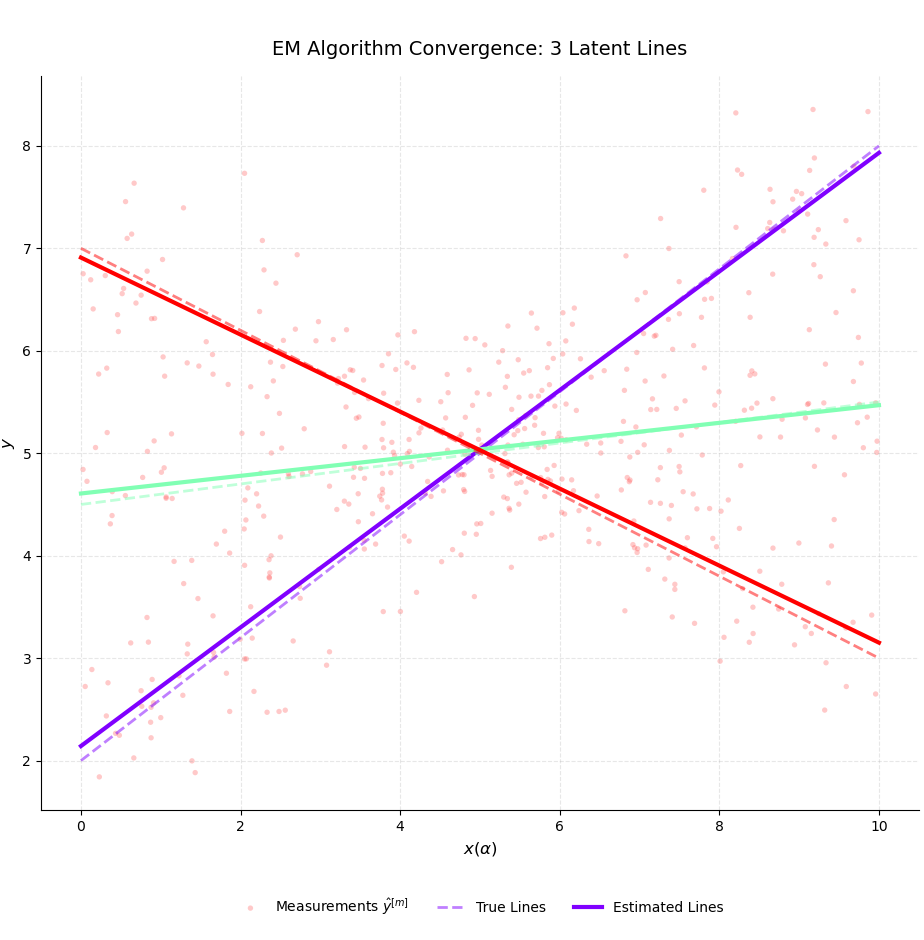
\includegraphics[width=\linewidth]{images/L1.png}
    \caption{Successful recovery of 3 latent lines.}
    \label{fig:l3}
\end{minipage}\hfill
\begin{minipage}{0.48\textwidth}
    \centering
    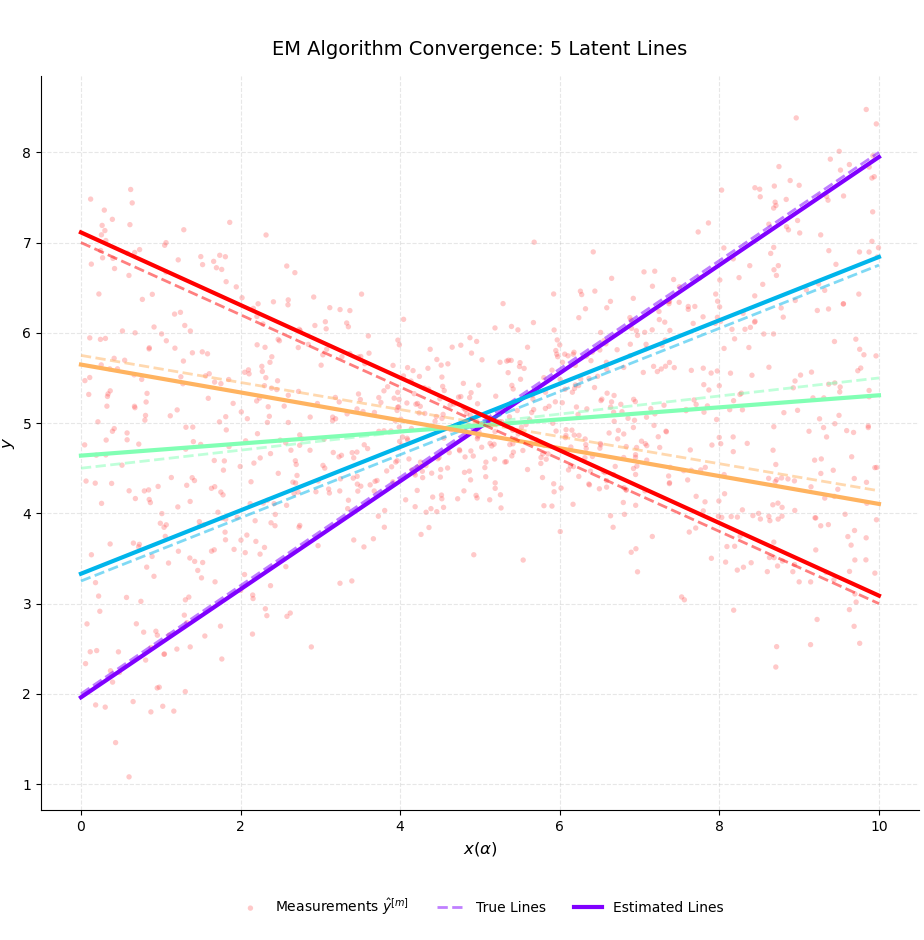
\includegraphics[width=\linewidth]{images/L5.png}
    \caption{Successful recovery of 5 latent lines.}
    \label{fig:l5}
\end{minipage}
\end{figure}

\begin{figure}[H]
\centering
\begin{minipage}{0.48\textwidth}
    \centering
    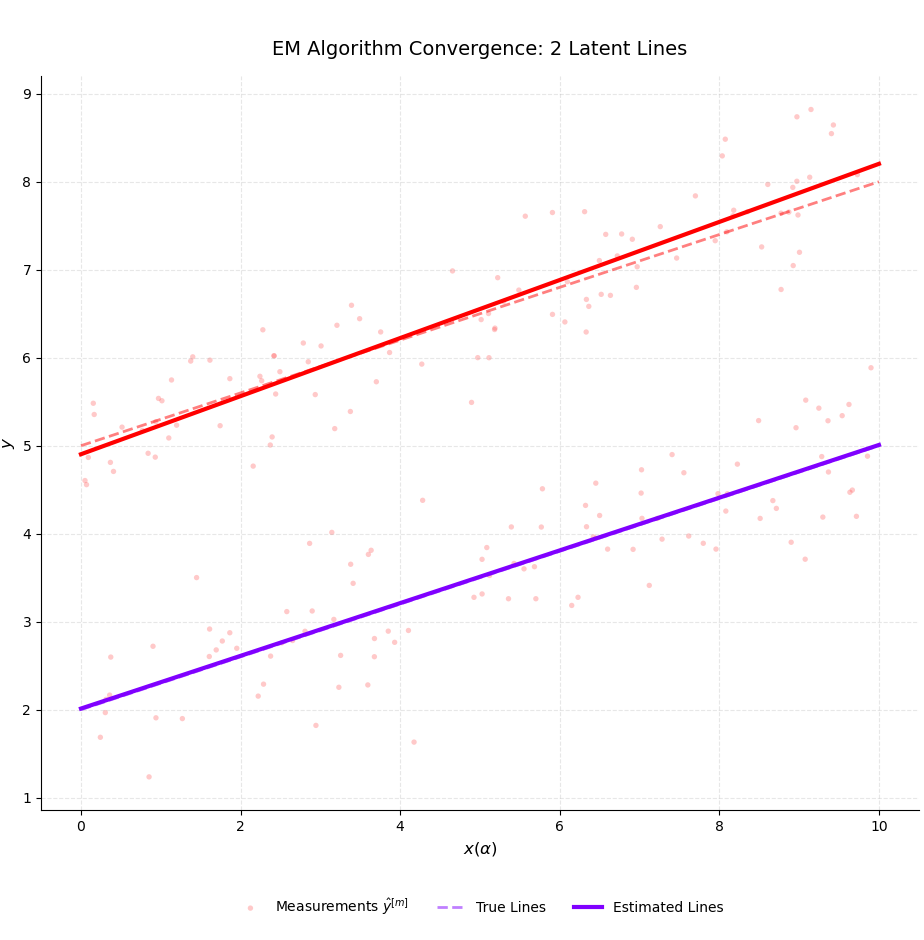
\includegraphics[width=\linewidth]{images/parallel.png}
    \caption{Success: Parallel data with parallel initialisation.}
    \label{fig:parallel_correct}
\end{minipage}\hfill
\begin{minipage}{0.48\textwidth}
    \centering
    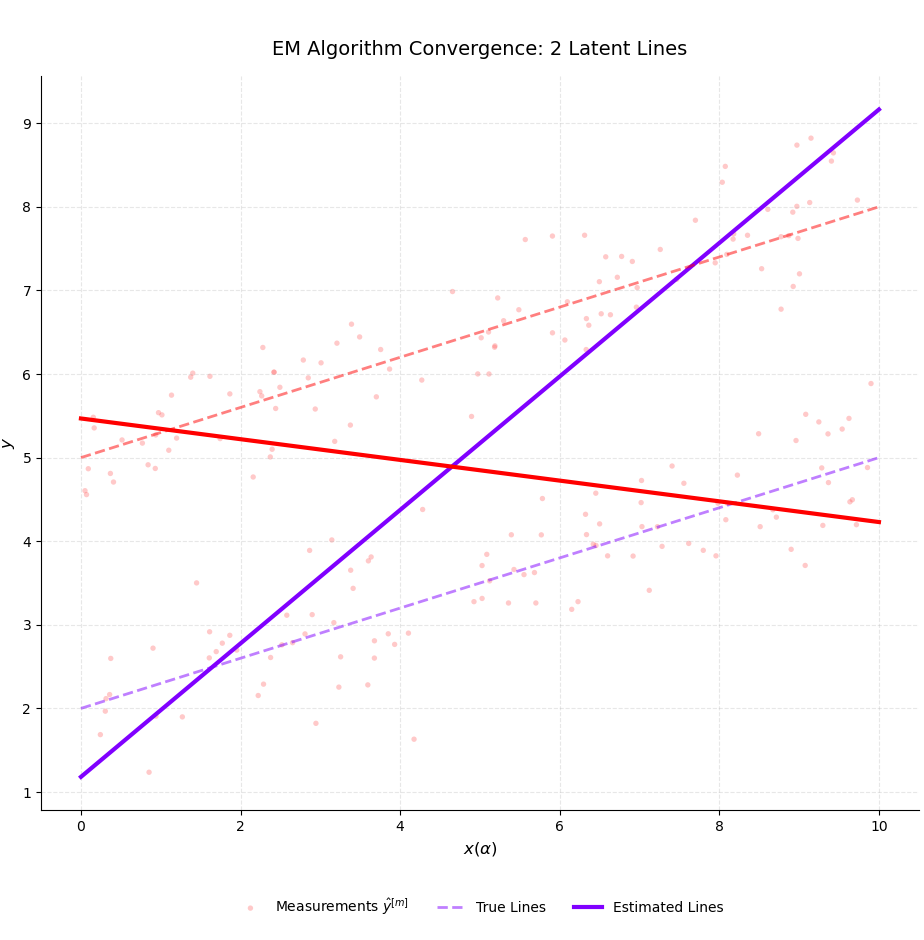
\includegraphics[width=\linewidth]{images/parallelwrong.png}
    \caption{Failure: Parallel data with crossing initialisation.}
    \label{fig:parallel_wrong}
\end{minipage}
\end{figure}

\end{document}